\let\negmedspace\undefined
\let\negthickspace\undefined
\documentclass[journal]{IEEEtran}
\usepackage[a5paper, margin=10mm, onecolumn]{geometry}
%\usepackage{lmodern} % Ensure lmodern is loaded for pdflatex
\usepackage{tfrupee} % Include tfrupee package

\setlength{\headheight}{1cm} % Set the height of the header box
\setlength{\headsep}{0mm}     % Set the distance between the header box and the top of the text

\usepackage{gvv-book}
\usepackage{gvv}
\usepackage{cite}
\usepackage{amsmath,amssymb,amsfonts,amsthm}
\usepackage{algorithmic}
\usepackage{graphicx}
\usepackage{textcomp}
\usepackage{xcolor}
\usepackage{txfonts}
\usepackage{listings}
\usepackage{enumitem}
\usepackage{mathtools}
\usepackage{gensymb}
\usepackage{comment}
\usepackage[breaklinks=true]{hyperref}
\usepackage{tkz-euclide} 
\usepackage{listings}
% \usepackage{gvv}                                        
\def\inputGnumericTable{}                                 
\usepackage[latin1]{inputenc}                                
\usepackage{color}                                            
\usepackage{array}                                            
\usepackage{longtable}                                       
\usepackage{calc}                                             
\usepackage{multirow}                                         
\usepackage{hhline}                                           
\usepackage{ifthen}                                           
\usepackage{lscape}
\begin{document}

\bibliographystyle{IEEEtran}
\vspace{3cm}

\title{1-1.6-14}
\author{AI24BTECH11010  - Golla Shriram
}
% \maketitle
% \newpage
% \bigskip
{\let\newpage\relax\maketitle}

\renewcommand{\thefigure}{\theenumi}
\renewcommand{\thetable}{\theenumi}
\setlength{\intextsep}{10pt} % Space between text and floats


\numberwithin{equation}{enumi}
\numberwithin{figure}{enumi}
\renewcommand{\thetable}{\theenumi}


\textbf{Question}:\\
     Points $\vec{A}(3,1), \vec{B}(12,-2)$  and $ \vec{C}(0,2) $ cannot be vertices of a triangle.  \\
\textbf{Solution: } \\
       If $\vec{A},\vec{B}$and $\vec{C}$ are collinear then they are not vertices of triangle.  \\
  Points $\vec{A},\vec{B},\vec{C} $ are defined to be collinear if \\
                                 \begin{align}  rank(\vec{B-A}  \  \vec{C-A} ) = 1 \end{align}
                                 The collinearity matrix  is \\
                          \begin{align}       \myvec{9 & -3 
                                 \\ -12 & 4} 
                                  \xleftrightarrow[]{R_2 \leftarrow {3R_2+4R_1}}
 \myvec{
   9 & -3 
   \\
   0 & 0
 }
 \end{align}
 
 By applying row reductions we get rank of matrix as 1. So, $\vec{A},\vec{B},\vec{C} $ are collinear.
\begin{figure}[h!]
   \centering
   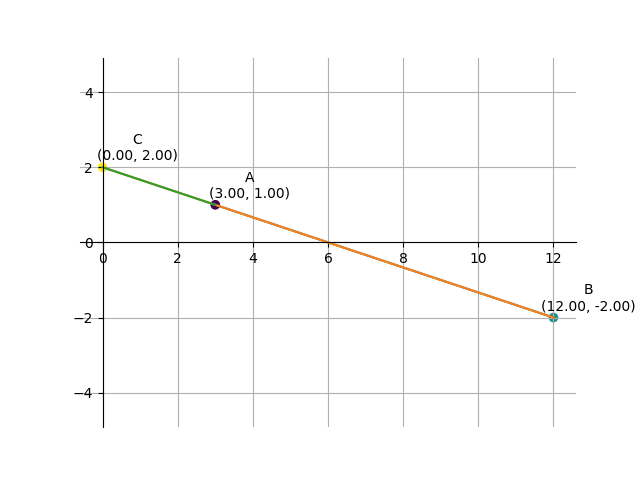
\includegraphics[width=0.7\linewidth]{figs/Figure_1.png}
	\caption{Plot of $\vec{A},\vec{B},\vec{C}$}
   \label{stemplot}
\end{figure}

\end{document}  
\end{document}


